%

\begin{figure}
    \centering
    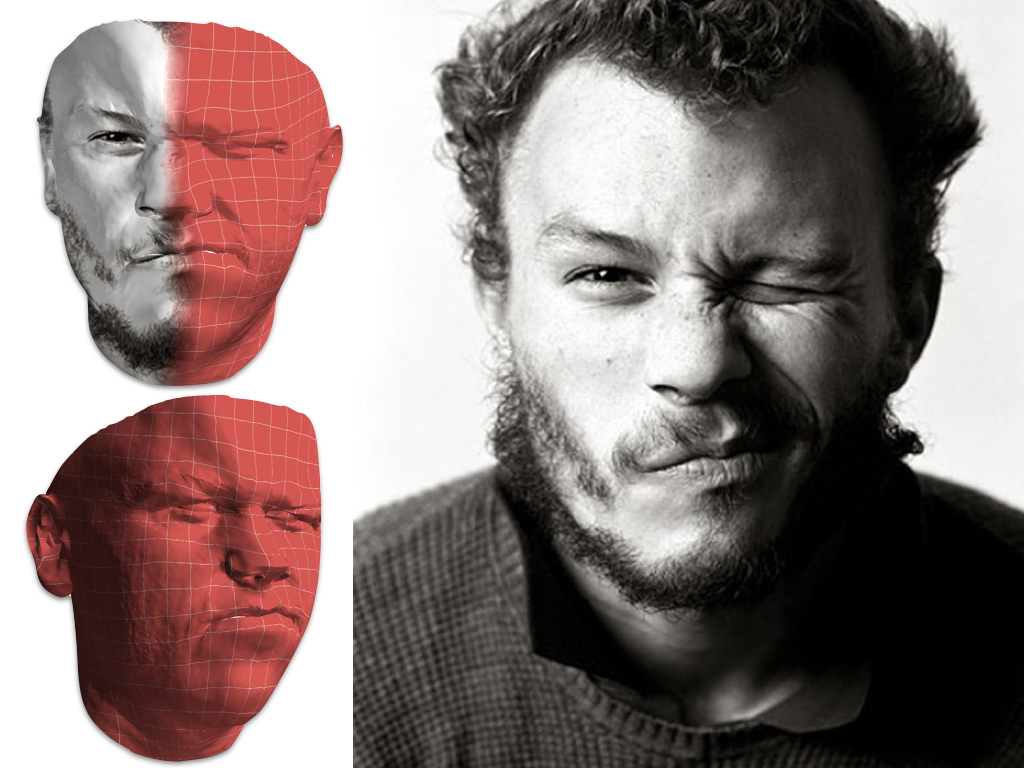
\includegraphics[width=\linewidth]{hero_figure}
    \caption{Our ``in-the-wild'' Morphable Model is capable of recovering accurate 3D facial shape for a wide variety of images.}
\label{fig:hero}
\end{figure}

\section{Introduction}
During the past few years, we have witnessed significant improvements in various
face analysis tasks such as face detection~\cite{fddbTech,zafeiriou2015survey}
and 2D facial landmark localization on static
images~\cite{xiong2013supervised,kazemi2014one,asthana2014incremental,tzimiropoulos2014gauss,zhu2015face,antonakos2015feature,antonakos2015active,trigeorgis2016mnemonic}.
This is primarily attributed to the fact that the community has made a
considerable effort to collect and annotate facial images
captured under unconstrained conditions~\cite{le2012interactive,zhu2012face,LFPW_belhumeur2013localizing,sagonas2013300,sagonas2016faces} (commonly referred to as ``in-the-wild'') and to the discriminative methodologies that can capitalise on the availability of
such large amount of data. Nevertheless, discriminative techniques cannot be
applied for 3D facial shape estimation ``in-the-wild'', due to lack of
ground-truth data.

3D facial shape estimation from single images has attracted the attention of
many researchers the past twenty years. The two main lines of research are \emph{(i)}~fitting a 3D Morphable Model
(3DMM)~\cite{blanz1999morphable,blanz2003face} and \emph{(ii)}~applying Shape from Shading (SfS) techniques~\cite{snape2015automatic,snape2014kernel,kemelmacher2013internet}.
The 3DMM fitting proposed in the work of
Blanz and Vetter~\cite{blanz1999morphable,blanz2003face} was among the first model-based 3D
facial recovery approaches. The method requires the construction of a 3DMM which
is a statistical model of facial texture and shape in a space where there are
explicit correspondences. The first 3DMM was built using 200 faces captured
in well-controlled conditions displaying only the neutral expression.
That is the reason why the method was only shown to work on real-world, but not ``in-the-wild'', images.
State-of-the-art SfS techniques capitalise on special multi-linear decompositions
that find an approximate spherical harmonic decomposition of the illumination.
Furthermore, in order to benefit from the large availability of ``in-the-wild'' images, these methods jointly reconstruct large collections of images. Nevertheless, even thought the results of \cite{snape2015automatic,kemelmacher2013internet} are quite interesting, given that there is no prior of the facial surface, the methods only recover 2.5D representations of the faces and particular smooth approximations of the facial normals.

3D facial shape recovery from a single image under ``in-the-wild'' conditions is still an open and challenging problem in computer vision mainly due to the fact that:
\begin{itemize}
\item The general problem of extracting the 3D facial shape from a single image
is an ill-posed problem which is notoriously difficult to be solved without the
use of any statistical priors for the shape and texture of faces. That is,
without prior knowledge regarding the shape of the object at-hand there are
inherent ambiguities present in the problem. The pixel intensity at a location
in an image is the result of a complex combination of the underlying shape of
the object, the surface albedo and normal characteristics, camera parameters
and the arrangement of scene lighting and other objects in the scene.
Hence, there are potentially infinite solutions to the problem.

\item Learning statistical priors of the 3D facial shape and texture for
``in-the-wild'' images is currently very difficult by using modern acquisition devices.
That is, even though there is a considerable improvement in 3D acquisition
devices, they still cannot operate in arbitrary conditions. Hence, all the
current 3D facial databases have been captured in controlled conditions.
\end{itemize}

With the available 3D facial data, it is feasible to learn a powerful statistical model of the facial shape that generalises well for both identity and expression \cite{cao2014facewarehouse,paysan20093d,booth3d}.
However, it is not possible to construct a statistical model of the facial texture that
generalises well for ``in-the-wild'' images and is, at the same time, in
correspondence with the statistical shape model.
That is the reason why current state-of-the-art 3D face reconstruction
methodologies rely solely on fitting a statistical 3D facial shape prior on a
sparse set of landmarks \cite{aldrian2013inverse,huber2015fitting}.

In this paper, we make a number of contributions that enable the use of 3DMMs for ``in-the-wild'' face reconstruction (Fig.~\ref{fig:hero}). In particular, our contributions are:

\begin{itemize}

\item We propose a methodology for learning a statistical texture model from ``in-the-wild'' facial images, which
is in full correspondence with a statistical shape prior that exhibits both
identity and expression variations.
Motivated by the success of feature-based
(e.g., HOG~\cite{dalal2005histograms}, SIFT~\cite{lowe1999object})
Active Appearance Models (AAMs)~\cite{antonakos2014hog,antonakos2015feature}
we further show how to learn feature-based texture models for 3DMMs.
We show that the advantage of using the ``in-the-wild'' feature-based texture model is that the fitting strategy gets simplified since there is not need to optimize with respect to the illumination parameters.

\item By capitalising on the recent advancements in fitting statistical
deformable models~\cite{papandreou2008adaptive,tzimiropoulos2013optimization,antonakos2015feature,alabort2016unified},
we propose a novel and fast algorithm for fitting ``in-the-wild'' 3DMMs. Furthermore, we make the
implementation of our algorithm publicly available, which we believe can be of
great benefit to the community, given the lack of robust open-source implementations for fitting 3DMMs.

\item Due to lack of ground-truth data, the majority of the 3D face
reconstruction papers report only qualitative results. In this paper, in order
to provide quantitative evaluations, we collected a new dataset of 3D facial surfaces, using Kinect Fusion~\cite{izadi2011kinectfusion,newcombe2011kinectfusion}, which has many ``in-the-wild'' characteristics, even though it is captured indoors.

\item We release an open source implementation of our technique as part of the Menpo Project.~\cite{menpo14}

\end{itemize}

The remainder of the paper is structured as follows.
In Section~\ref{sec:training} we elaborate on the construction of our ``in-the-wild'' 3DMM,
whilst in Section~\ref{sec:fitting} we outline the proposed optimization for fitting
``in-the-wild'' images with our model. Section~\ref{sec:dataset} describes our
new dataset, the first of its kind, to provide images with a ground-truth 3D facial shape that exhibit many ``in-the-wild'' characteristics. We outline a series of quantitative and qualitative experiments in Section~\ref{sec:experiments}, and end with conclusions in Section~\ref{sec:conclusion}.


%

%





%


%
%

%
%
%
%

%


%
%

%
%


%
%
%
